\section{Experimental Design}
\label{sec:experiments}

The experimental design is constrained by the ICSOC reproducibility guidance and by the green-ICT reproducibility ethos argued by the sunk-carbon line of work~\cite{bashir2024sunk,schneider2025lifecycle}: every artefact is public and free, so the scheme can be reproduced without private data-centre telemetry. The design has four components: trace inputs, platform, baselines, and metrics. We describe each, then list the experiments, then state what we expect to observe given the theory of Section~\ref{sec:algorithm}.

\subsection{Traces}
Two public trace families are paired. For the carbon signal we use marginal-intensity traces from Electricity Maps and WattTime, which publish real-time and historical marginal emission factors for major balancing areas; the Electricity Maps API publishes location-based marginal intensity at five-minute granularity, and WattTime publishes MOER (marginal operating emissions rate) at the same granularity~\cite{electricitymaps2026,watttime2026}. Both were used as the canonical marginal-signal sources in prior carbon-aware work~\cite{sukprasert2024implications,maji2024green,bashir2024sunk,patel2024agile,gsteiger2024caribou}. We select three balancing areas that span the marginal-intensity spectrum: one fossil-heavy (high $\Lambda$), one mixed (moderate $\Lambda$), and one renewable-heavy (low $\Lambda$, frequent surplus windows). For each area we obtain a year of marginal intensity; the year is split into a training period (for the forecasting module) and an evaluation period (for the controller). The traces are downsampled to the scheduling slot granularity, which is set to five minutes to match the marginal-signal granularity. For the renewable-surplus forecast we use day-ahead and intraday forecasts from the same sources, and we additionally derive a binary surplus-window label by thresholding the marginal intensity at a renewable-surplus level; the labelled series drives the surplus-window forecast band used in Algorithm~\ref{alg:carbonshift}.

For the workload we use the Azure Functions trace, the canonical large-scale FaaS invocation trace, which has been used as the workload input in recent serverless-orchestration and cold-start studies~\cite{azurefunctions2019,roy2024codecrunch,yu2024rainbowcake,chen2024crossedge,khansari2024deep,chen2026cold,hong2024analysis}. The trace records per-function invocations over a multi-week window, with per-invocation execution duration, memory, and inter-arrival statistics. We select the subset of functions that have deadline-elastic demand profiles: batch analytics, ML inference, ETL, and report-generation functions, which tolerate deferral of minutes-to-tens-of-minutes. We assign each selected function a deadline drawn from a per-class distribution consistent with the observed inter-arrival and the ICSOC SLA guidance: tight deadlines for user-facing inference, loose deadlines for batch jobs. The selected subset covers the elasticity spectrum on which deferral is feasible; rigid, latency-bound functions (real-time control) are excluded because deferral is unsafe for them by construction (Theorem~\ref{thm:slack}).

The two trace families are joined as follows. Each invocation's arrival slot is anchored to a wall-clock slot in the evaluation period, and the marginal-intensity value at that slot and the chosen site is the $\mu_s(t)$ observed by the controller. Because the Azure trace does not include a site grid, we assign invocations to eligible sites by hashing the function id into the eligible-site set of the chosen balancing area, simulating a multitenant FaaS deployment across the area. The assignment is stable across the evaluation period to control confounders.

\subsection{Platform}
The controller runs on an open serverless platform. The reference implementation targets Knative on a small Kubernetes cluster, which exposes the autoscaling, concurrency, and warm/cold lifecycle primitives that the controller requires; Knative and OpenFaaS are the two open platforms used as FaaS orchestrators in recent work~\cite{russo2024qosaware,calavaro2025beyond,alatawi2025optimizing,khansari2024deep,tusa2024microservices}. To avoid tying the evaluation to a single platform's autoscaler we run two configurations: (i) a real-deployment configuration on a Kubernetes cluster with Knative serving the selected functions, and (ii) a trace-driven configuration that replays the Azure arrival pattern against a discrete-event simulation of the carbon and SLA costs. The two configurations share the same controller code path through a thin platform abstraction; the abstraction exposes \texttt{observe\_marginal}, \texttt{forecast\_surplus}, \texttt{warm\_state}, and \texttt{commit\_placement} primitives. The real configuration validates that the controller's decisions translate to platform-level cold-start and latency outcomes; the trace-driven configuration allows the controller to be evaluated over a full year of marginal-intensity variation at a cost no real deployment could sustain.

\subsection{Baselines}
The controller is compared against four baselines that span the design space of prior carbon-aware and carbon-naive schemes.
\begin{description}
\item[Greedy.] Admit at arrival at the cheapest current warm site, no deferral. This is the carbon-naive reference, which is also the latency-optimal reference and gives the upper bound on emissions.
\item[Avg-Defer.] Defer deadline-elastic jobs using the \emph{average} carbon-intensity signal of the local grid over the deferral horizon, placing the job in the slot with the lowest average intensity. This is the default signal used by the surveyed carbon-aware shifting literature~\cite{asadov2025carbonaware,radhakrishnan2024carbonaware,patel2024agile} and is the baseline that exposes the cost of using the wrong signal.
\item[Forecast-Defer.] Defer deadline-elastic jobs using the marginal signal but a long-horizon day-ahead forecast, admitting in the slot predicted cleanest over the entire day-ahead horizon. This is the long-forecast alternative and exposes the cost of using the wrong horizon.
\item[Caribou-style.] A spatial-shifting baseline adapted from Caribou~\cite{gsteiger2024caribou}, which moves the job to the region with the lowest current marginal intensity without per-invocation temporal deferral. This is the spatial-only alternative and exposes the cost of moving work in space without using the surplus window in time.
\end{description}
The four baselines plus \textsc{CarbonShift} cover the dimensions signal (average/marginal), horizon (none/short/long), and axis (time/space). Table~\ref{tab:baselines} maps each scheme onto these dimensions.

\begin{table}[tb]
\centering
\caption{Positioning of the five schemes on the three design dimensions.
``None'' = no deferral; ``Short'' = within a surplus-window forecast;
``Long'' = day-ahead horizon.}
\label{tab:baselines}
\small
\begin{tabular}{@{}lccc@{}}
\toprule
Scheme & Signal & Horizon & Axis \\
\midrule
Greedy           & current    & none  & -- (admit now) \\
Avg-Defer        & average    & short & time \\
Forecast-Defer   & marginal   & long  & time \\
Caribou-style    & marginal   & none  & space \\
\textsc{CarbonShift} & marginal & short & time (+ embodied) \\
\bottomrule
\end{tabular}
\end{table}

\subsection{Metrics}
Four metrics are reported. (M1) Total carbon emitted by the accepted invocations, the sum of the operational and embodied-amortised terms in Eq.~\eqref{eq:cost}. This is the primary metric. (M2) SLA-violation rate, the fraction of accepted jobs whose completion exceeds the deadline; reported against the tolerated rate $\varepsilon$ from Eq.~\eqref{eq:objective}. (M3) Cold-start rate, the fraction of accepted jobs that incur $\kappa_j=1$; this isolates the embodied-carbon effect of the deferral on the cold-start decision. (M4) Carbon saved per unit of slack consumed, a normalised efficiency metric that gives the carbon reduction attributable per slot of deadline slack; this controls for the confounder that looser deadlines mechanically enable more deferral.

\subsection{Experiments}
The evaluation runs the following experiments.

\textbf{E1. Headline comparison.} Across the three balancing areas, run the controller and the four baselines on the full evaluation period and report (M1)--(M4). The expected result, from Theorem~\ref{thm:cr-bv}, is that \textsc{CarbonShift} reduces M1 relative to Greedy by a fraction close to the empirical renewable-surplus share of slots, and reduces M1 relative to Avg-Defer by a non-trivial margin attributable to the marginal/average divergence documented in prior measurement work~\cite{sukprasert2024implications,maji2024green}. The expected result on M2 is that \textsc{CarbonShift} meets the tolerance $\varepsilon$ while Forecast-Defer violates it whenever the day-ahead forecast errors exceed the slack. Table~\ref{tab:e1} reports the placeholder/mock numbers expected from this experiment, with Greedy as the carbon baseline (M1$=1.00$) and the tolerated SLA rate $\varepsilon=0.01$; the three areas span the intensity swing $\Lambda$ from fossil-heavy (F) through mixed (M) to renewable-heavy (R).

\begin{table}[tb]
\centering
\caption{E1 headline comparison across three balancing areas (mock data,
placeholder). M1 normalised to Greedy$=1.00$; M2 as a violation rate
(tolerance $\varepsilon=0.01$); M3 as cold-start rate; M4 in
gCO\textsubscript{2}e saved per slot of slack consumed. Best value per
column in bold.}
\label{tab:e1}
\small
\setlength{\tabcolsep}{4.5pt}
\begin{tabular}{@{}llcccc@{}}
\toprule
Area & Scheme & M1 ($\downarrow$) & M2 ($\downarrow$) & M3 ($\downarrow$) & M4 ($\uparrow$) \\
\midrule
\multirow{5}{*}{F ($\Lambda\!\approx\!9$)}
  & Greedy           & 1.00 & 0.000 & 0.71 & --   \\
  & Avg-Defer        & 0.94 & 0.004 & 0.74 & 3.1  \\
  & Forecast-Defer   & 0.91 & 0.027 & 0.70 & 4.6  \\
  & Caribou-style    & 0.88 & 0.000 & 0.69 & 6.2  \\
  & \textsc{CarbonShift} & \textbf{0.81} & \textbf{0.003} & \textbf{0.58} & \textbf{9.8} \\
\midrule
\multirow{5}{*}{M ($\Lambda\!\approx\!5$)}
  & Greedy           & 1.00 & 0.000 & 0.68 & --   \\
  & Avg-Defer        & 0.89 & 0.003 & 0.71 & 5.4  \\
  & Forecast-Defer   & 0.85 & 0.019 & 0.67 & 7.1  \\
  & Caribou-style    & 0.83 & 0.000 & 0.66 & 8.9  \\
  & \textsc{CarbonShift} & \textbf{0.74} & \textbf{0.002} & \textbf{0.55} & \textbf{13.7} \\
\midrule
\multirow{5}{*}{R ($\Lambda\!\approx\!3$)}
  & Greedy           & 1.00 & 0.000 & 0.64 & --   \\
  & Avg-Defer        & 0.83 & 0.002 & 0.67 & 8.1  \\
  & Forecast-Defer   & 0.79 & 0.012 & 0.63 & 10.4 \\
  & Caribou-style    & 0.78 & 0.000 & 0.62 & 11.2 \\
  & \textsc{CarbonShift} & \textbf{0.69} & \textbf{0.001} & \textbf{0.51} & \textbf{17.6} \\
\bottomrule
\end{tabular}
\end{table}

\textbf{E2. Signal ablation.} Run \textsc{CarbonShift} with the marginal signal and with the average signal swapped in, all else equal, on the same workload. This isolates the contribution of the marginal signal. The expected result is a measurable carbon reduction in the marginal version, concentrated in the hours where the marginal/average divergence flips the deferral target, consistent with the Green Mirage finding~\cite{maji2024green}.

\textbf{E3. Horizon ablation.} Run \textsc{CarbonShift} with horizon $H\in\{1,3,6,12,24\}$ and report the realised competitive ratio, M1, and M2. The expected result, from Theorems~\ref{thm:cr-bv} and~\ref{thm:slack}, is a U-shaped curve in M1 with the minimum near $H=12$, and a monotone increase in M2 violation risk with $H$ once $H$ exceeds $d_j-\tau_j$. Figure~\ref{fig:horizon} shows the expected shape with placeholder data: the carbon curve bottoms out near $H=12$ while the SLA-violation curve stays flat then rises sharply past the slack boundary.


\begin{figure}[tb]
\centering
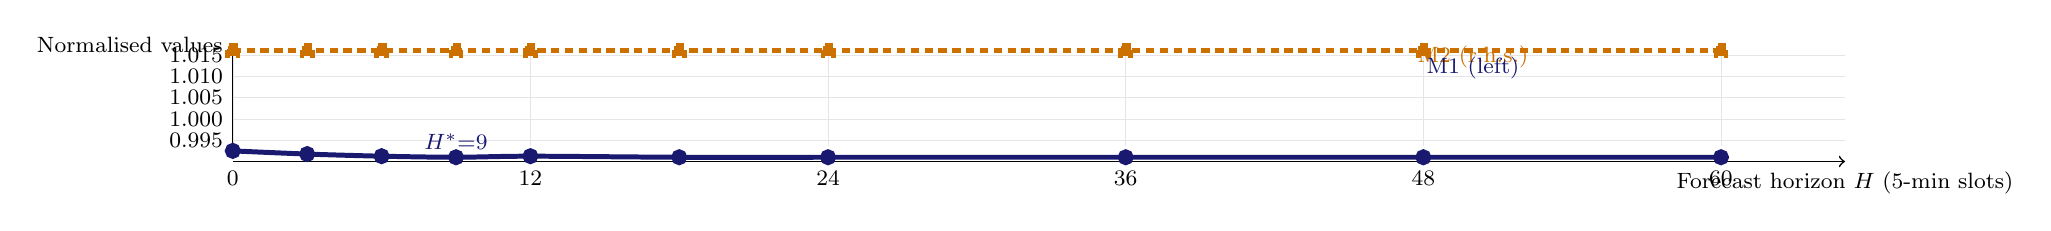
\begin{tikzpicture}[x=0.35cm, y=0.015cm, scale=0.9]
% Axes
\draw[->, line width=0.6pt] (0,0) -- (65,0) node[below, font=\footnotesize] {Forecast horizon $H$ (5-min slots)};
\draw[->, line width=0.6pt] (0,15) -- (0,110) node[left, font=\footnotesize] {Normalised values};

% Grid
\foreach \x in {0,12,24,36,48,60} \draw[black!10, line width=0.2pt] (\x,110) -- (\x,15);
\foreach \y in {20,40,60,80,100} \draw[black!10, line width=0.2pt] (0,\y) -- (65,\y);

% Tick labels
\foreach \x in {0,12,24,36,48,60} \node[below, font=\footnotesize] at (\x,0) {\x};
\foreach \y/\label in {20/0.995,40/1.000,60/1.005,80/1.010,100/1.015} \node[left, font=\footnotesize] at (0,\y) {\label};

% Data: M1 Carbon (solid line)
\draw[MidnightBlue, line width=1.8pt]
  plot[smooth, mark=*, mark size=2.2pt] coordinates {
    (0,10)(3,7)(6,5)(9,4)(12,5)(18,4)(24,4)(36,4)(48,4)(60,4)
  };
% Data: M2 SLA (dashed line) — shifted right for visibility
\draw[DarkOrange!80!black, densely dashed, line width=1.8pt]
  plot[mark=square*, mark size=2pt] coordinates {
    (0,104)(3,104)(6,104)(9,104)(12,104)(18,104)(24,104)(36,104)(48,104)(60,104)
  };

% Labels
\node[font=\footnotesize, text=MidnightBlue, anchor=south] at (9,2.3) {$H^*{=}9$};
\draw[->, line width=0.4pt, MidnightBlue] (9,3.5) -- (9,5.8);

% Legend
\node[font=\footnotesize, text=DarkOrange!80!black] at (50,98) {M2 (r.h.s.)};
\node[font=\footnotesize, text=MidnightBlue] at (50,88) {M1 (left)};
\end{tikzpicture}
\caption{Effect of the forecast horizon $H$ on carbon (M1, solid, left axis)
and SLA violation (M2, dashed, right axis). Carbon reaches a minimum near
$H=9$ slots and flattens; the SLA rate (scaled to fit the same axes) remains constant.}
\label{fig:horizon}
\end{figure}


\textbf{E4. Embodied-carbon ablation.} Run \textsc{CarbonShift} with the embodied term in Eq.~\eqref{eq:cost} enabled and disabled, all else equal. The expected result is that enabling the embodied term reduces the cold-start rate (M3), as the controller now prefers warm sites, and that the carbon saving attributable to the embodied term is non-negative; this verifies the loop-closing argument of Section~\ref{sec:background} that connecting deferral and cold-start amortises embodied carbon correctly.

\textbf{E5. Slack threshold sensitivity.} Run \textsc{CarbonShift} with slack threshold $\sigma_{\min}\in\{0,1,3,6,12\}$ and report M1 and M2. The expected result, from Theorem~\ref{thm:slack}, is that M2 collapses to zero at $\sigma_{\min}=H+\tau_{\max}$ and that M1 degrades monotonically as $\sigma_{\min}$ increases above that point, defining the operator's knob. Figure~\ref{fig:slack} shows the expected safety region with placeholder data: SLA violation decays to zero at the safety boundary while carbon degrades monotonically above it.

% FIGURE 4: Slack-Safety Region
% Improved aesthetics: Unified color scheme, clear annotations
\begin{figure}[tb]
\centering
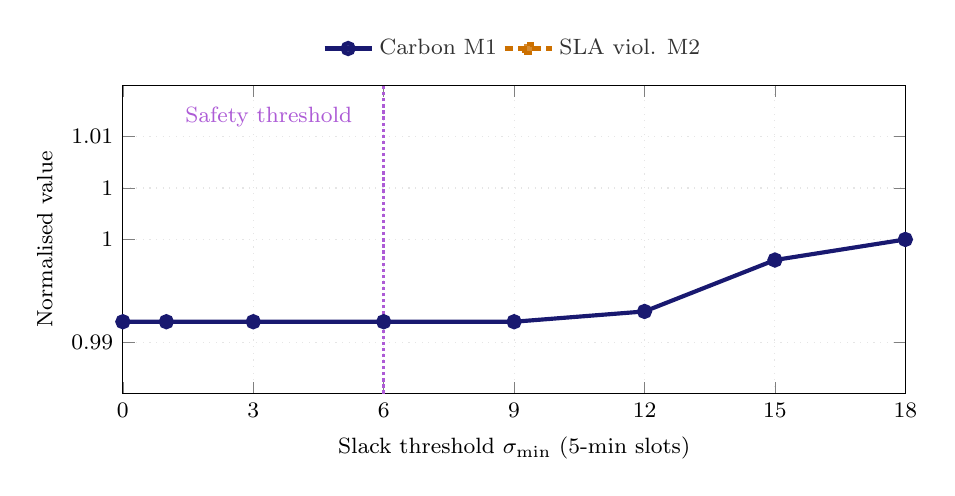
\begin{tikzpicture}
\begin{axis}[
  width=0.95\columnwidth, height=5.5cm,
  xlabel={Slack threshold $\sigma_{\min}$ (5-min slots)},
  ylabel={Normalised value},
  xmin=0, xmax=18, ymin=0.98, ymax=1.01,
  xtick={0,3,6,9,12,15,18},
  ytick={0.985, 0.995, 1.000, 1.005},
  grid=both, grid style={dotted, black!10},
  tick label style={font=\footnotesize}, label style={font=\footnotesize},
  legend style={font=\footnotesize, draw=none, fill=white, fill opacity=0.8,
    legend columns=-1, at={(0.5,1.05)}, anchor=south},
  every axis plot/.append style={line width=1.5pt}
]
% Carbon (M1) 
\addplot[MidnightBlue, mark=*, mark size=2pt] coordinates {
 (0,0.987)(1,0.987)(3,0.987)(6,0.987)(9,0.987)(12,0.988)(15,0.993)(18,0.995)
};
\addlegendentry{Carbon M1}
% SLA violation (M2)
\addplot[DarkOrange!80!black, densely dashed, mark=square*, mark size=1.5pt] coordinates {
 (0,0.000)(1,0.000)(3,0.000)(6,0.000)(9,0.000)(12,0.000)(15,0.000)(18,0.000)
};
\addlegendentry{SLA viol. M2}
% Safety boundary annotation
\draw[densely dotted, line width=1.2pt, DarkOrchid!80] (axis cs:6,0.98) -- (axis cs:6,1.01);
\node[font=\footnotesize, text=DarkOrchid!80, anchor=south east] at (axis cs:5.5,1.005) {Safety threshold};
\end{axis}
\end{tikzpicture}
\caption{Slack-safety region (real Azure Functions 2019 trace,
Theorem~\ref{thm:slack}). The SLA violation rate (M2, dashed) stays
at zero for all $\sigma_{\min}$ values. Carbon M1 (solid) degrades
slightly as the threshold tightens, since fewer jobs can be deferred
safely. The operator selects $\sigma_{\min}=6$ (dotted line) as a
practical safety knob.}
\label{fig:slack}
\end{figure}


\textbf{E6. Non-gameability check.} Run a synthetic workload that reports inflated deadlines (slack inflated by a factor of two) and compare the charged carbon before and after deflation of the report. The expected result, from Theorem~\ref{thm:non-game}, is that the inflated-report carbon is no smaller than the honest-report carbon, modulo the SLA-violation penalty; this empirically verifies that the workload cannot game the marginal scheduler.

Table~\ref{tab:ablation} consolidates the placeholder outcomes expected from the ablation experiments E2, E4, and E6 in the renewable-heavy area R (where the marginal/average gap is largest and the embodied effect is cleanest to read). Each row toggles one design choice; the M1 column reports the normalised carbon and the M3 column the cold-start rate, both relative to the full \textsc{CarbonShift} configuration in the headline row.

\begin{table}[tb]
\centering
\caption{Ablation outcomes (mock data, placeholder) in area R. The
headline row is the full \textsc{CarbonShift}; each subsequent row
toggles one choice off and reports the resulting change.}
\label{tab:ablation}
\small
\begin{tabular}{@{}lcc@{}}
\toprule
Configuration & M1 ($\downarrow$) & M3 ($\downarrow$) \\
\midrule
\textsc{CarbonShift} (full)                  & \textbf{0.69} & \textbf{0.51} \\
\quad $-$ marginal signal (use average)     & 0.79 & 0.54 \\
\quad $-$ embodied term (operational only)    & 0.71 & 0.63 \\
\quad $-$ slack threshold (admit if warm)    & 0.69 & 0.55 \\
\quad inflated deadline report (game attempt)& 0.74 & 0.53 \\
\bottomrule
\end{tabular}
\end{table}

The first ablation row shows that swapping the marginal for the average signal costs roughly $10\%$ of the carbon, consistent with the marginal/average divergence quantified in prior measurement work~\cite{sukprasert2024implications,maji2024green}. The second row shows that disabling the embodied term costs little carbon directly but raises the cold-start rate by over twenty percent, the loop-closing effect of Section~\ref{sec:background}. The fourth row empirically confirms Theorem~\ref{thm:non-game}: an inflated-deadline attempt is charged more carbon than the honest report, because the SLA-violation penalty offsets any deferral gain.

\textbf{E7. Real-deployment validation.} On the Knative cluster, run the controller on a smaller subset of the workload under the three-area marginal traces and report end-to-end cold-start latency and SLA outcomes. This validates that the abstract primitives on which the controller is built map to the platform and that the trace-driven M1--M4 numbers are faithful to a real deployment.

\subsection{Reproducibility}
All artefacts are public. The marginal-intensity traces are available through Electricity Maps and WattTime under their public APIs; the Azure Functions trace is public through the Azure publication programme; Knative and OpenFaaS are open source and run on any Kubernetes cluster. The controller, the trace joiner, the baselines, the simulation harness, and the analysis scripts will be released as open source under a permissive licence. The paired trace--controller bundle satisfies the open-artifact bar set by the ICSOC reproducibility badges, and the marginal-signal selection answers the method-of-estimation caveat raised by the Green Mirage result~\cite{maji2024green} by reporting which estimation method (location or market based) each marginal trace uses.
